%\centerline{
%\begin{minipage}{\widefigwidth}
\resizebox{\textwidth}{!}{
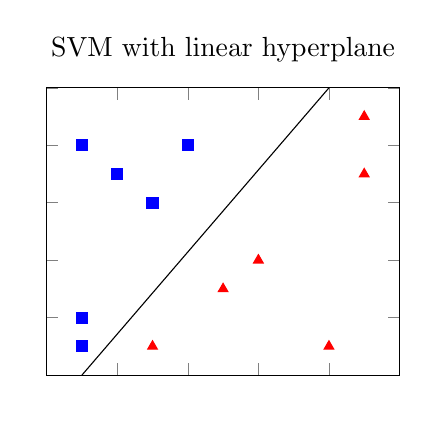
\begin{tikzpicture}
\begin{axis}[
    title={SVM with linear hyperplane},
    width=.5\textwidth,
    xmin=0, xmax=10,
    ymin=0, ymax=10,
    %xtick={0,...,10},
    yticklabels={,,},
    xticklabels={,,},
]
\addplot[
    color=blue,
    mark=square*,
    only marks,
    ]
    coordinates {
    (1,1) (1,2) (1,8) (2,7) (4,8) (3,6)
    };
\addplot[
    color=red,
    mark=triangle*,
    only marks
    ]
    coordinates {
    (3,1) (8,1) (5,3) (6,4) (9,7) (9,9)
    };
\addplot[
    color=black,
    ]
    coordinates{
    (1,0) (8,10)
    };
\end{axis}
\end{tikzpicture}
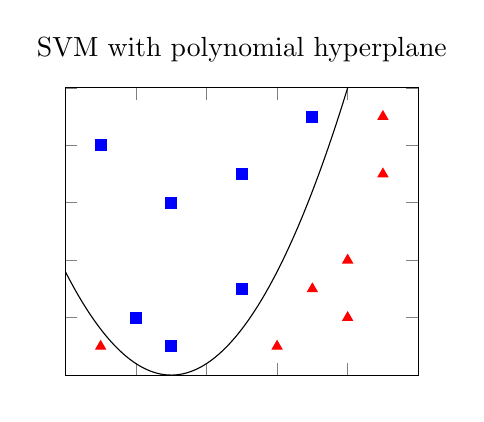
\begin{tikzpicture}
\begin{axis}[
    title={SVM with polynomial hyperplane},
    width=.5\textwidth,
    xmin=0, xmax=10,
    ymin=0, ymax=10,
    %xtick={0,...,10},
    yticklabels={,,},
    xticklabels={,,},
]
\addplot[
    color=blue,
    mark=square*,
    only marks,
    ]
    coordinates {
    (3,1) (2,2) (1,8) (5,7) (7,9) (3,6) (5,3)
    };
\addplot[
    color=red,
    mark=triangle*,
    only marks
    ]
    coordinates {
    (1,1) (6,1) (8,2) (7,3) (8,4) (9,7) (9,9)
    };
\addplot[
    color=black,
    domain=0:10,
    samples=100] (\x,{0.4*(\x-3)^2});
\end{axis}
\end{tikzpicture}
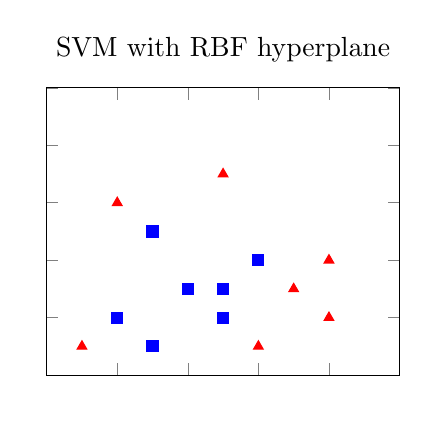
\begin{tikzpicture}
\begin{axis}[
    title={SVM with RBF hyperplane},
    width=.5\textwidth,
    xmin=0, xmax=10,
    ymin=0, ymax=10,
    %xtick={0,...,10},
    yticklabels={,,},
    xticklabels={,,},
]
\addplot[
    color=blue,
    mark=square*,
    only marks,
    ]
    coordinates {
    (3,1) (2,2) (5,2) (4,3) (6,4) (3,5) (5,3)
    };
\addplot[
    color=red,
    mark=triangle*,
    only marks
    ]
    coordinates {
    (1,1) (6,1) (8,2) (7,3) (8,4) (5,7) (2,6)
    };
\draw (axis cs:4,3) circle [black, radius=25];
\end{axis}
\end{tikzpicture}
%\end{minipage}
}